\chapter{The arithmetic question}
\label{chap:g01-question}

\section{A group and a field have different obligations}

A finite group can be written down in many ways. A multiplication table gives all its products. A permutation representation gives an action on a finite set. Matrices give linear operators whose compositions obey the same law. Each description makes the symmetry concrete. The inverse Galois problem asks for a further kind of realization, one that has to exist inside arithmetic.

\begin{conjecture}[Inverse Galois over the rational numbers]
\label{conj:g01-igp}
For every finite group $G$, there is a finite Galois extension $L/\Q$ and an isomorphism
\[
G\simeq\Gal(L/\Q).
\]
\end{conjecture}

The quantifiers matter. The ground field is the same $\Q$ for every group. The extension $L$ may depend on $G$. It must be a field, its degree must be finite, and all its automorphisms over $\Q$ must form exactly the prescribed group. An embedding of $G$ into a larger Galois group does not satisfy the conclusion. Nor does an extension over a convenient field that changes with the group.

The trivial group causes no difficulty. Take $L=\Q$. For a nontrivial group, a realization has degree
\begin{equation}
\label{eq:g01-degree}
[L:\Q]=|G|.
\end{equation}
This is a consequence of the finite Galois theorem, rather than a definition of the target. A field of degree $|G|$ need not be Galois and need not have $|G|$ automorphisms. Degree and symmetry are separate tests until normality and separability have been established.

\begin{figure}[tbp]
\centering
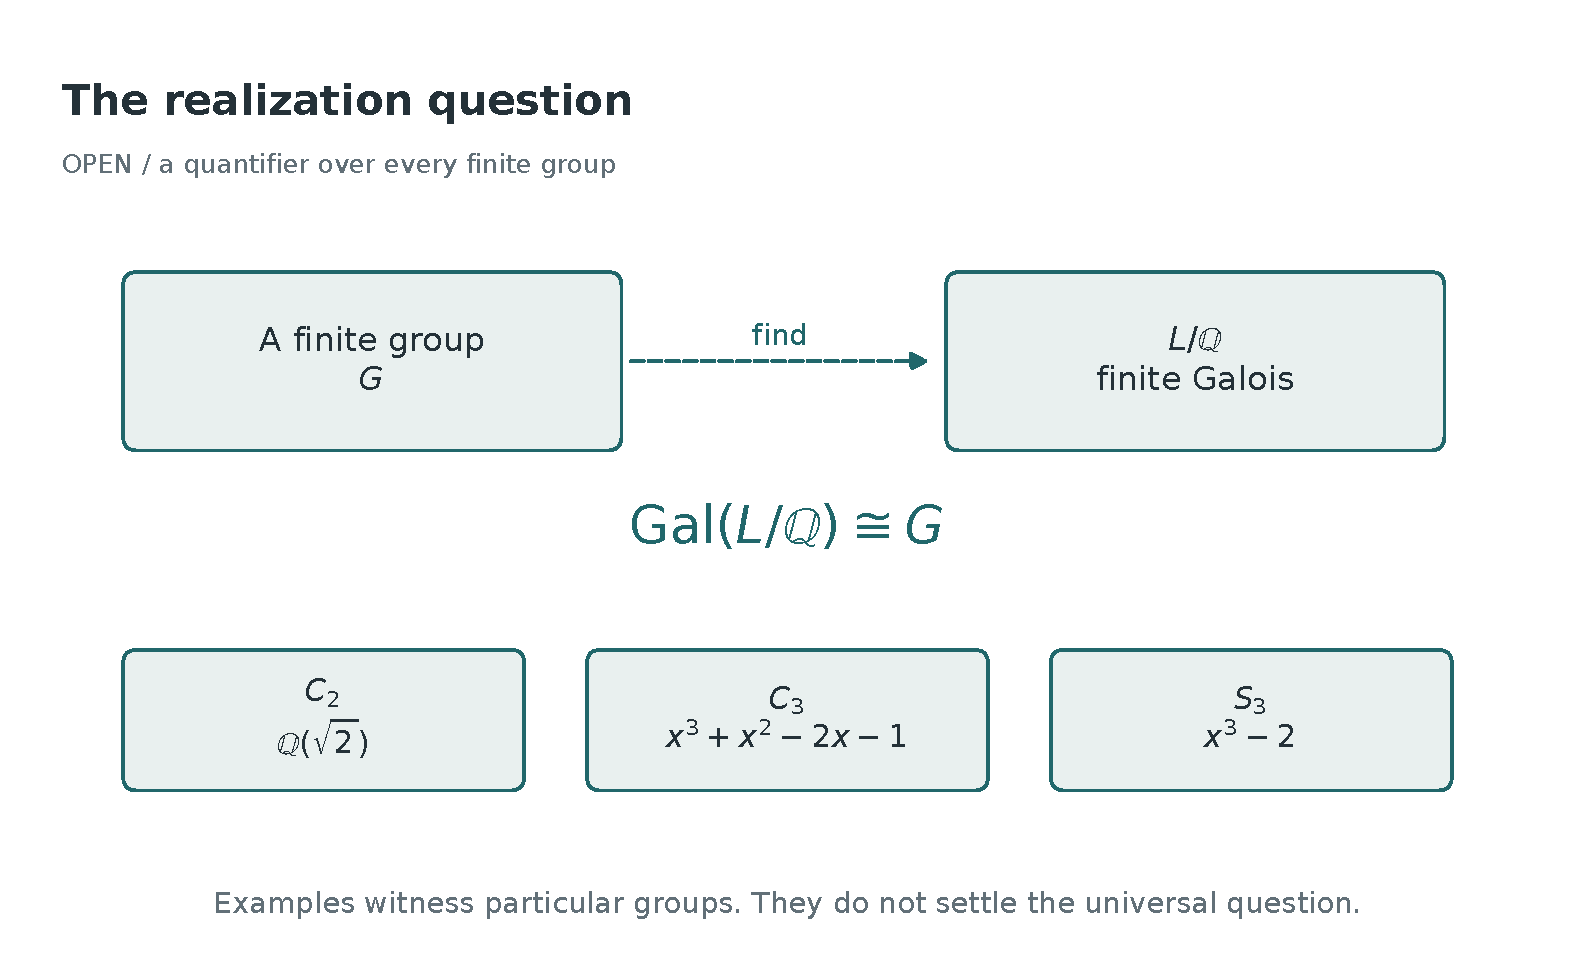
\includegraphics[width=0.96\linewidth]{../visual/figures/01_goal.pdf}
\caption{The inverse problem starts with a prescribed finite group and requires a finite Galois field extension over the fixed ground field $\Q$. A representation of the group supplies symmetry data. Arithmetic realization must additionally supply the field and its full automorphism group.}
\label{fig:g01-goal}
\end{figure}

\section{Why the splitting field is the relevant object}

Let $f\in\Q[X]$ be a nonconstant polynomial. A splitting field is a smallest field extension in which $f$ is a product of linear factors. It is unique up to an isomorphism that fixes $\Q$. In characteristic zero, every irreducible polynomial is separable. The splitting field of $f$ is therefore a finite Galois extension, even if $f$ itself is reducible or has repeated factors. Replacing $f$ by the product of its distinct irreducible factors does not change this field.

If $\alpha$ is just one root, the field $\Q(\alpha)$ can be smaller than the splitting field. The remaining roots need not lie in it. The equation $X^3-2=0$ will give our first explicit example of this distinction. Its real root generates a field of degree three, whereas the field containing all three roots has degree six.

\begin{proposition}[An equivalent polynomial formulation]
\label{prop:g01-polynomial}
Conjecture~\ref{conj:g01-igp} is equivalent to the following assertion. Every finite group is the Galois group of the splitting field over $\Q$ of some separable polynomial in $\Q[X]$.
\end{proposition}

\begin{proof}
A splitting field in characteristic zero is finite Galois, so the polynomial assertion gives the field assertion. Conversely, let $L/\Q$ be finite Galois. The primitive element theorem gives $L=\Q(\alpha)$ for some $\alpha$. Its minimal polynomial is separable. Normality says that every conjugate of $\alpha$ over $\Q$ belongs to $L$. Thus $L$ contains the splitting field. The splitting field also contains $\alpha$ and hence all of $L$, so the two fields agree. The primitive element theorem used here is a classical input for finite separable extensions \cite{Milne2022}.
\end{proof}

An integral polynomial can be used if desired. Clear denominators to obtain a polynomial in $\Z[X]$ with the same roots. The resulting polynomial need not be monic. Alternatively, multiply a primitive element by an integer large enough to make it integral and use its monic minimal polynomial. These changes concern presentation. They do not replace the requirement that the splitting field have the correct group.

\section{The action on roots}

Suppose $f$ has $d$ distinct roots in its splitting field $L$. Every automorphism of $L/\Q$ permutes them. The action is faithful because the roots generate $L$: an automorphism fixing every root fixes every rational expression in those roots. Consequently
\begin{equation}
\label{eq:g01-root-action}
\Gal(L/\Q)\hookrightarrow S_d.
\end{equation}
If $f$ is irreducible, the action is transitive. One way to see this is to send any root to any other through the isomorphism between the corresponding simple extensions, then extend that embedding to the splitting field. Normality ensures that the resulting embedding is an automorphism of $L$. This standard extension theorem is included in the finite Galois framework \cite{Milne2022}.

Transitivity does useful work. The orbit of a root has size $d$, so the order of the group is divisible by $d$. It does not identify the group by itself. A cubic can have group $C_3$ or $S_3$. A quartic can have several transitive subgroups of $S_4$. The examples in the next chapter show how extra information selects the group.

\begin{figure}[tbp]
\centering
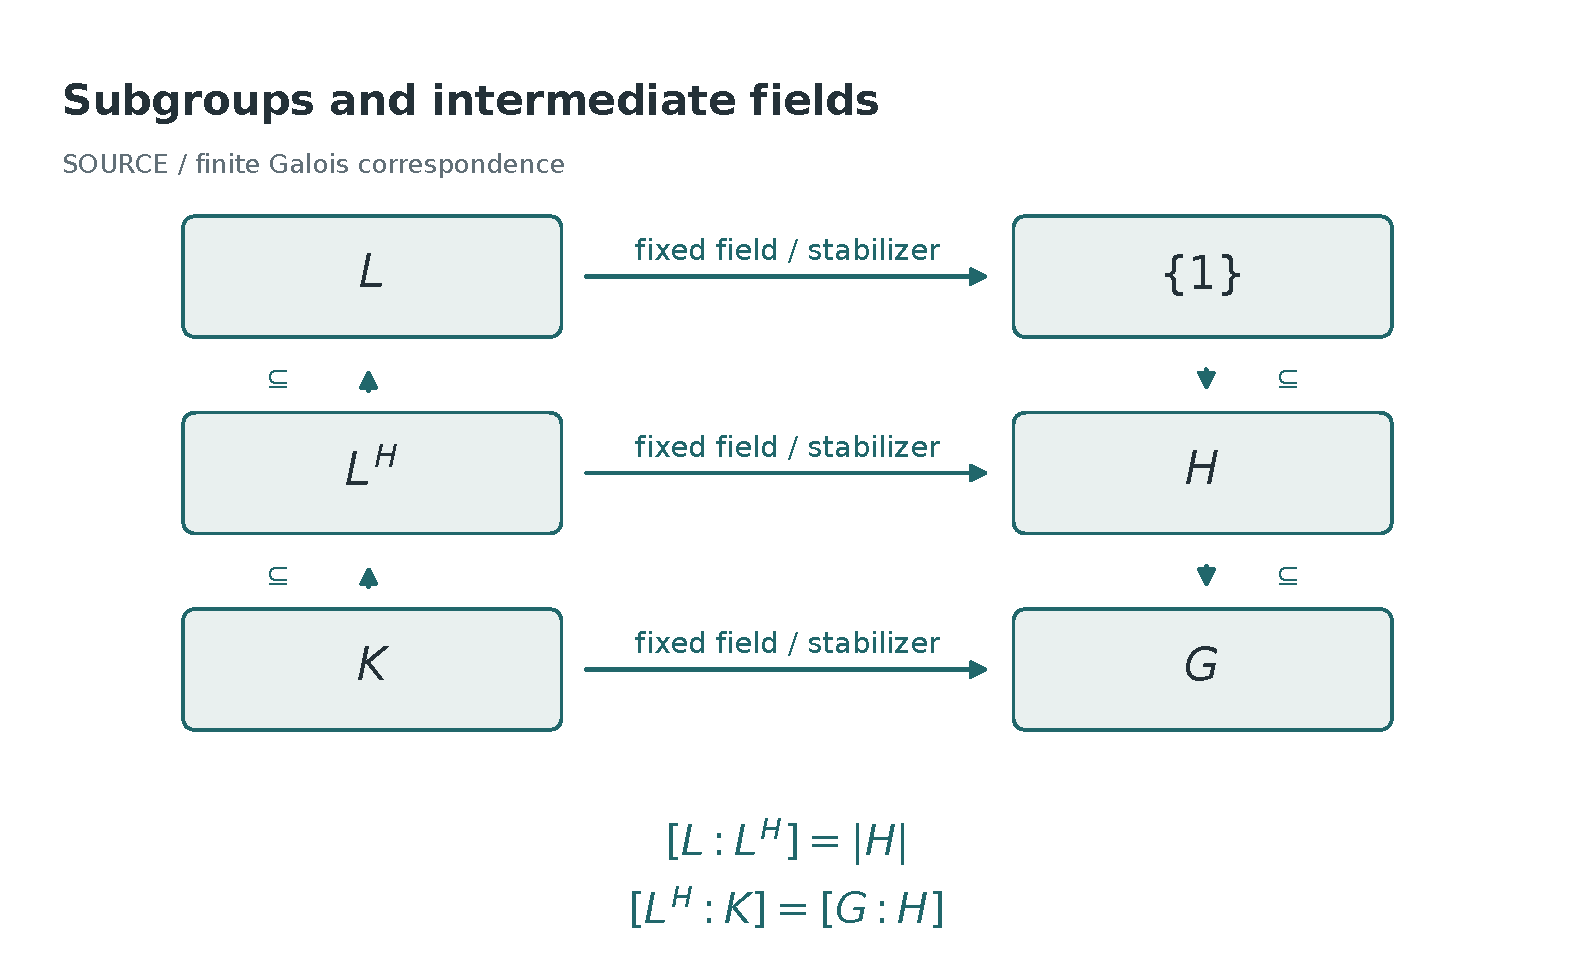
\includegraphics[width=0.96\linewidth]{../visual/figures/02_field_group.pdf}
\caption{For an already supplied finite Galois extension $L/K$ with group $G$, subgroups $H\le G$ correspond to intermediate fixed fields $L^H$. The direction of inclusion reverses. The classical correspondence computes degrees and organizes fields after the ambient field extension has been established \cite[Theorem 3.17]{Milne2022}.}
\label{fig:g01-field-group}
\end{figure}

\section{The regular representation supplies a model}

Let $G$ be any finite group. Its left regular action is the permutation action on its own underlying set,
\[
g\cdot h=gh.
\]
It is faithful: if $g$ fixes the identity element, then $g=1$. On the vector space $\Q^G$ with basis $e_h$, the corresponding operators are
\[
\rho(g)e_h=e_{gh}.
\]
They satisfy $\rho(g_1g_2)=\rho(g_1)\rho(g_2)$ and give an embedding $G\hookrightarrow\operatorname{GL}(\Q^G)$. These are exact constructions for every finite group.

They do not yet give an extension of $\Q$. The vector space $\Q^G$ has no designated field multiplication. Its coordinatewise multiplication makes it a product algebra, which has zero divisors whenever $|G|>1$. For distinct $h,k$, the coordinate idempotents satisfy $e_he_k=0$ although both are nonzero. A finite product of copies of $\Q$ is a useful algebraic symmetry model, but it cannot be the required nontrivial number field.

A proposed rational bilinear multiplication would only begin the next test. It must be commutative and associative, have a unit and have no zero divisors. In finite dimension these properties make it a field: multiplication by a nonzero element is an injective linear map and hence is surjective, so the element has an inverse. The action must also preserve that multiplication. Then one must prove that the fixed field is $\Q$ and that the full automorphism group is the chosen $G$. The finite automorphism theorem can discharge the last group calculation once an actual field and actual field automorphisms are available. It does not manufacture those inputs.

\begin{claimboundary}
Faithful permutation and matrix realizations exist for every finite group. They prove that finite symmetry can be represented exactly. The inverse Galois conjecture asks whether that symmetry can always be realized as the full automorphism group of a finite field extension of $\Q$.
\end{claimboundary}

This distinction will remain central when projector packets and transfer operators enter the discussion. Such structures can preserve information about a group action or about an extension already supplied. They have to carry additional arithmetic construction data before they can prove that a new extension exists. The following examples supply genuine fields, not only representations.

\chapter{Five complete field realizations}
\label{chap:g02-examples}

\section{Quadratic symmetry: $C_2$}

Let $\alpha=\sqrt2$ and $L=\Q(\alpha)$. The polynomial $X^2-2$ is irreducible over $\Q$. Indeed, if $a/b$ in lowest terms had square two, then $a^2=2b^2$ would make $a$ even. Writing $a=2c$ gives $b^2=2c^2$, so $b$ would also be even, a contradiction.

Every element of $L$ has a unique expression $a+b\alpha$ with $a,b\in\Q$. The map
\[
\sigma(a+b\alpha)=a-b\alpha
\]
preserves addition and multiplication because both $\alpha$ and $-\alpha$ satisfy the same relation $\alpha^2=2$. It fixes $\Q$, has square the identity, and is nontrivial. The only possible images of $\alpha$ under a rational automorphism are $\alpha$ and $-\alpha$. Thus there are exactly two automorphisms.

The polynomial already splits in $L$, so $L/\Q$ is Galois and
\[
\Gal(L/\Q)=\{1,\sigma\}\simeq C_2.
\]
Its fixed elements satisfy $a+b\alpha=a-b\alpha$, whence $b=0$. This directly checks $L^{\langle\sigma\rangle}=\Q$ without appealing to an abstract correspondence. The same argument works for every nonsquare $d\in\Q^\times$, with $\sqrt2$ replaced by $\sqrt d$.

\section{Two independent signs: $V_4$}

Now take
\[
L=\Q(\sqrt2,\sqrt3).
\]
The second square root does not belong to $\Q(\sqrt2)$. If $\sqrt3=a+b\sqrt2$, squaring and comparing the rational and $\sqrt2$ parts gives $2ab=0$ and $a^2+2b^2=3$. If $b=0$, a rational square would be three. If $a=0$, a rational square would be $3/2$. Neither is possible, as the prime exponents in a rational square are even. Thus the tower has degrees two and two, and $[L:\Q]=4$.

The four elements
\[
1,\quad\sqrt2,\quad\sqrt3,\quad\sqrt6
\]
form a rational basis. Independent choices of signs define four automorphisms. Let $s$ change the sign of $\sqrt2$ and let $t$ change the sign of $\sqrt3$. They satisfy
\[
s^2=t^2=1,\qquad st=ts.
\]
They are distinct because their effects on the two generators are distinct. The extension is the splitting field of $(X^2-2)(X^2-3)$, so it is Galois. Since the degree is four, these four automorphisms are the full group:
\[
\Gal(L/\Q)\simeq C_2\times C_2=V_4.
\]

\begin{figure}[tbp]
\centering
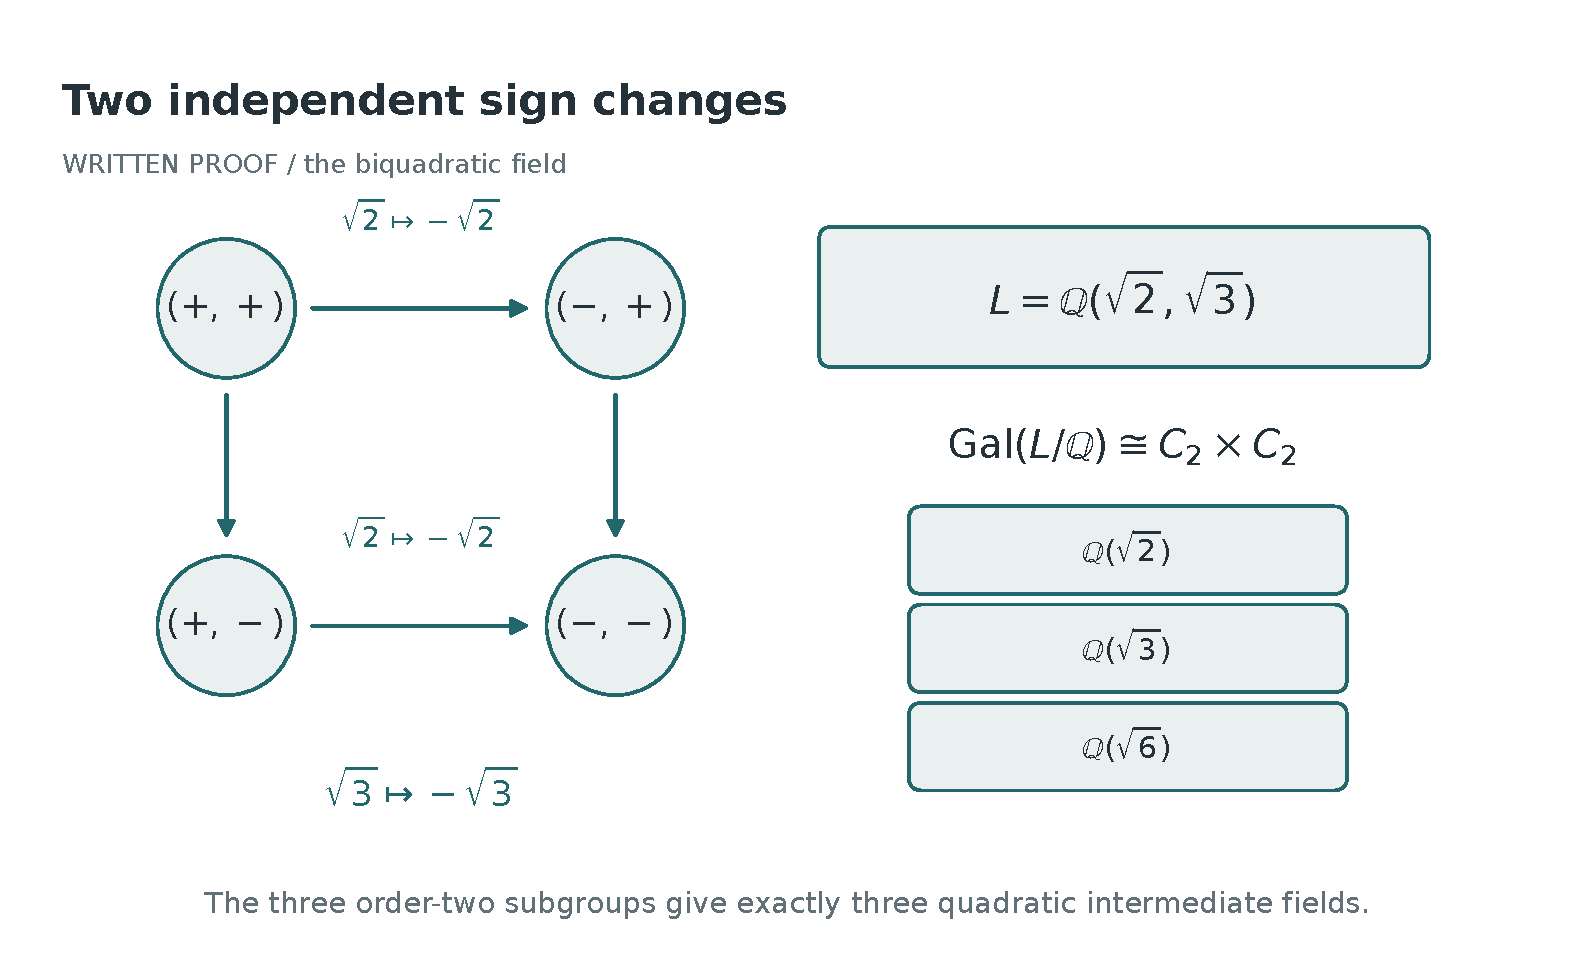
\includegraphics[width=0.96\linewidth]{../visual/figures/04_biquadratic.pdf}
\caption{The biquadratic field has three quadratic intermediate fields. Their sign symmetries give the three subgroups of order two in $V_4$. The degree calculations and fixed elements are proved directly in the text.}
\label{fig:g02-biquadratic}
\end{figure}

The fixed fields can also be read directly from the basis. The elements fixed by $s$ are $a+c\sqrt3$, so $L^{\langle s\rangle}=\Q(\sqrt3)$. Similarly, $L^{\langle t\rangle}=\Q(\sqrt2)$. The product $st$ changes the signs of both square roots but fixes their product, giving $L^{\langle st\rangle}=\Q(\sqrt6)$. An element fixed by both $s$ and $t$ has only its rational component left.

This example already exhibits a later theme. Averaging the operators $1$ and $s$ keeps the $1$ and $\sqrt3$ components while removing the other two. That operation recognizes a fixed subspace in a field already constructed. The proof that this subspace is the quadratic field $\Q(\sqrt3)$ uses the multiplication inherited from $L$.

\section{A cyclic cubic with discriminant $49$}

Consider
\[
f(X)=X^3+X^2-2X-1.
\]
The rational root theorem restricts rational roots to $1$ and $-1$. Since $f(1)=-1$ and $f(-1)=1$, there is no rational root. A reducible cubic over a field has a linear factor, so $f$ is irreducible.

For a monic cubic $X^3+aX^2+bX+c$, the discriminant is
\[
a^2b^2-4b^3-4a^3c-27c^2+18abc.
\]
Here this gives
\begin{equation}
\label{eq:g02-cubic-disc}
\operatorname{disc}(f)=4+32+4-27+36=49.
\end{equation}
The discriminant is nonzero, so the roots are distinct.

We can see the splitting field without using the discriminant criterion. Let $\alpha$ be a root. In $\Q(\alpha)$, the defining equation gives
\[
\alpha^3=-\alpha^2+2\alpha+1,
\qquad
\alpha^4=3\alpha^2-\alpha-1.
\]
Set
\[
\beta=\alpha^2-2,
\qquad
\gamma=-\alpha^2-\alpha+1.
\]
Direct reduction by the two displayed identities gives
\begin{equation}
\label{eq:g02-three-roots}
\alpha+\beta+\gamma=-1,
\quad
\alpha\beta+\alpha\gamma+\beta\gamma=-2,
\quad
\alpha\beta\gamma=1.
\end{equation}
Thus
\[
f(X)=(X-\alpha)(X-\beta)(X-\gamma)
\quad\text{in }\Q(\alpha)[X].
\]
For example, the second identity follows from
\[
\alpha(\beta+\gamma)=-\alpha-\alpha^2,
\qquad
\beta\gamma=\alpha^2+\alpha-2.
\]
The third follows by multiplying the latter expression by $\alpha$ and using the cubic relation. These are exact algebraic equalities, not numerical root approximations.

Since $f$ is irreducible, $[\Q(\alpha):\Q]=3$. Since it splits there, the root field is already its splitting field. Its Galois group has order three and is therefore cyclic. There is an explicit generator sending $\alpha$ to $\beta$. The map is well defined because $\beta$ is another root of the same irreducible polynomial. It is a field embedding into $\Q(\alpha)$ and hence an automorphism, since the image has degree three. The identities
\[
\beta^2-2=\gamma,
\qquad
\gamma^2-2=\alpha
\]
show that this automorphism cycles the three roots. Their distinctness also follows from the nonzero discriminant.

\begin{figure}[tbp]
\centering
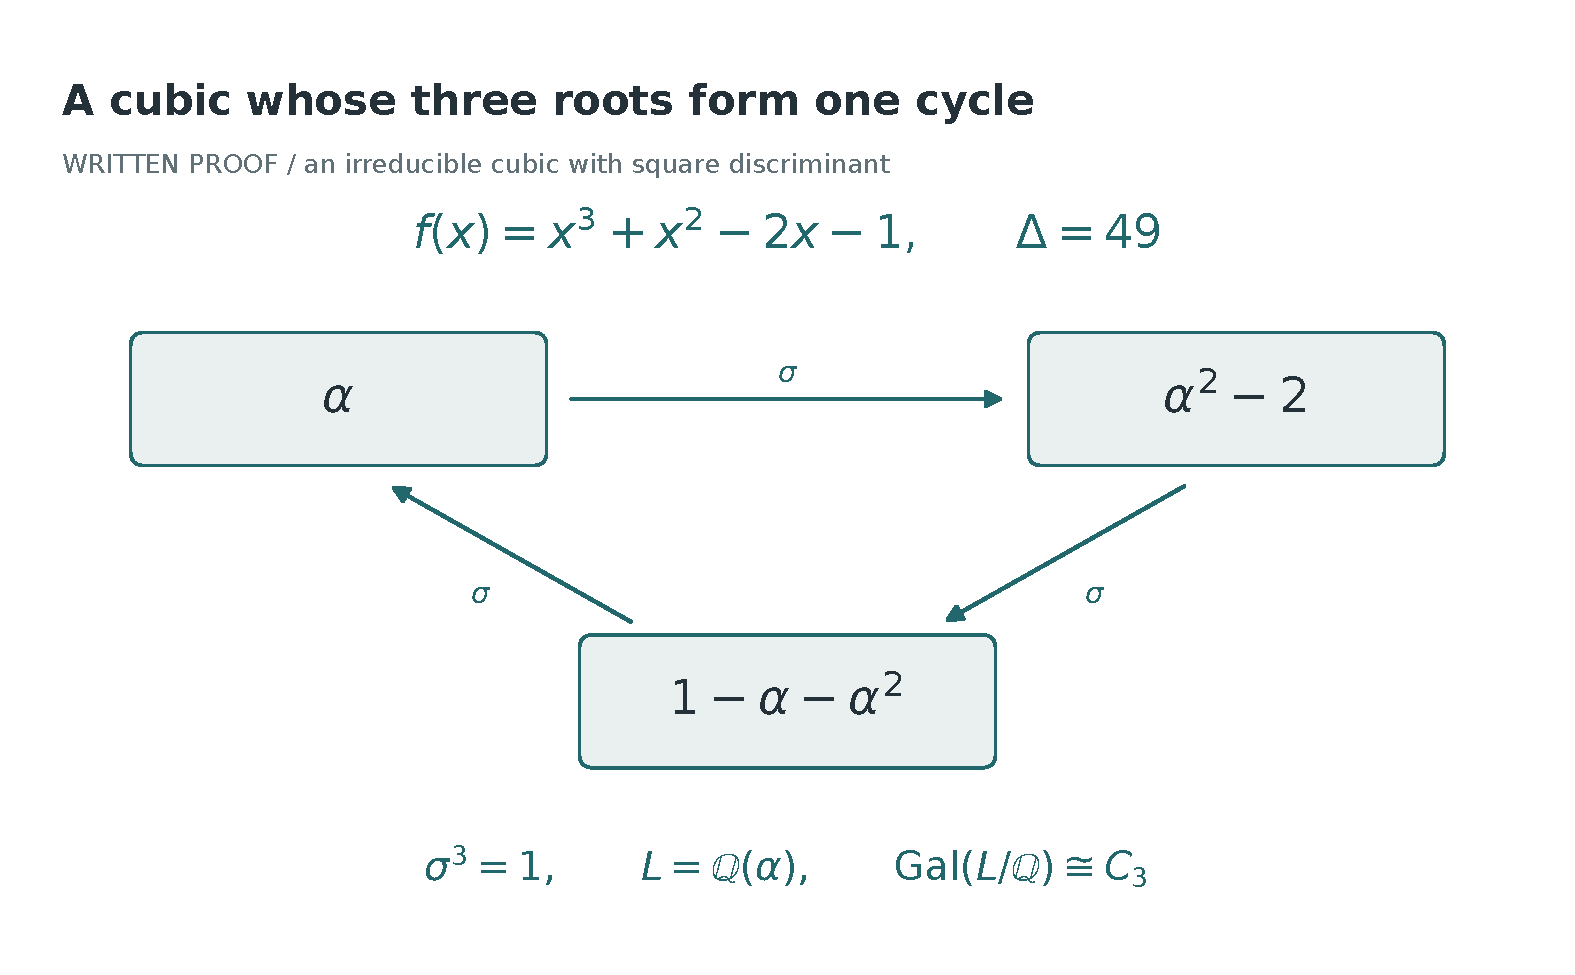
\includegraphics[width=0.96\linewidth]{../visual/figures/05_cyclic_cubic.pdf}
\caption{The cubic realization closes inside one root field. The transformation $r\mapsto r^2-2$ cycles its three roots, and their exact symmetric identities recover the original polynomial. The group has order three because the polynomial is irreducible and already splits in that field.}
\label{fig:g02-cyclic-cubic}
\end{figure}

The discriminant offers a second group check. If $r_1,r_2,r_3$ are the roots, the Vandermonde product $V=\prod_{i<j}(r_i-r_j)$ satisfies $V^2=49$. In a field of characteristic zero, this implies $V=7$ or $V=-7$, so every rational automorphism fixes $V$. Permuting the roots multiplies $V$ by the sign of the permutation. The group is therefore contained in $A_3$. Irreducibility makes it transitive, forcing it to be $A_3\simeq C_3$. This is a useful cross check of the explicit field computation. The figure labels the discriminant itself by $\Delta$, so $V^2=\Delta$.

\section{A cubic whose root field is too small: $S_3$}

Take $f(X)=X^3-2$ and let $\alpha$ denote its positive real root. Eisenstein's criterion at the prime two proves that $f$ is irreducible. Equivalently, a rational root would have to be an integer divisor of two, and none has cube two. Let $\zeta$ be a primitive cube root of unity, so
\[
\zeta^2+\zeta+1=0.
\]
The three roots are $\alpha,\zeta\alpha,\zeta^2\alpha$. Their splitting field is
\[
L=\Q(\alpha,\zeta).
\]
Indeed, this field contains every root, and the ratio of the second root to the first recovers $\zeta$ from the splitting field.

The field $\Q(\alpha)$ is contained in $\R$, whereas $\zeta$ is nonreal. Thus $\zeta\notin\Q(\alpha)$. Its quadratic equation remains irreducible over this real field, and
\begin{equation}
\label{eq:g02-s3-degree}
[L:\Q]=[L:\Q(\alpha)]\,[\Q(\alpha):\Q]=2\cdot3=6.
\end{equation}
The faithful action on three roots embeds $\Gal(L/\Q)$ into $S_3$. Both groups have order six, so the embedding is an isomorphism.

There is also a concrete pair of generators. Over $\Q(\zeta)$, the element $\alpha$ has degree three: the tower degree is $[L:\Q(\zeta)]=3$. Sending $\alpha$ to $\zeta\alpha$ while fixing $\zeta$ therefore gives an automorphism $\tau$ of order three. Complex conjugation gives an automorphism $c$ of order two that fixes $\alpha$ and sends $\zeta$ to $\zeta^2$. On the generators,
\[
c\tau c=\tau^{-1}.
\]
Hence the cyclic cubic subgroup is inverted by the other generator, as in the usual presentation of $S_3$.

The discriminant is $-108$. In particular it is not a square in $\Q$, agreeing with the presence of odd permutations. The degree calculation is already a complete proof, so the discriminant is corroborating information rather than an extra hypothesis. This separation prevents the example from becoming dependent on every possible way of recognizing its group.

\section{A quartic with cycle certificates: $S_4$}

For a quartic realization, consider
\[
f(X)=X^4-X-1.
\]
Its reduction modulo two is $X^4+X+1$. It has no root in $\mathbf F_2$. The only monic irreducible quadratic over $\mathbf F_2$ is $X^2+X+1$. Modulo that polynomial, $X^2=X+1$, $X^3=1$ and $X^4=X$, so $X^4+X+1$ has remainder one. A reducible quartic without a linear factor must factor as two irreducible quadratics. This possibility has just been excluded, proving that the reduction is irreducible. Gauss's lemma now proves that $f$ is irreducible over $\Q$.

We use one classical bridge between modular factorization and a characteristic zero group.

\begin{theorem}[Good prime cycle theorem, external input]
\label{thm:g02-cycle}
Let $f\in\Z[X]$ be monic, and suppose its reduction modulo a prime $p$ is squarefree. If its irreducible factors over $\mathbf F_p$ have degrees $d_1,\ldots,d_r$, the Galois group of its splitting field over $\Q$, acting on the roots of $f$, contains a permutation with disjoint cycle lengths $d_1,\ldots,d_r$.
\end{theorem}

This is the Frobenius factorization theorem in the stated squarefree setting \cite[Theorem 4.28]{Milne2022}. The theorem is external. The polynomial identities and the following finite irreducibility checks are displayed explicitly, so their role does not depend on trusting a numerical group label returned by software.

Modulo two, irreducibility gives a four cycle. Squarefreeness holds since the derivative of $X^4+X+1$ is one. Modulo seven there is the exact factorization
\begin{equation}
\label{eq:g02-mod-seven}
f(X)=(X-3)(X^3+3X^2+2X+5)
\quad\text{in }\mathbf F_7[X].
\end{equation}
The cubic takes the following values:
\[
\begin{array}{c|rrrrrrr}
x&0&1&2&3&4&5&6\\\hline
x^3+3x^2+2x+5\pmod7&5&4&1&2&6&5&5.
\end{array}
\]
It has no root, hence is irreducible. Its derivative $3X^2+6X+2$ is nonzero and has smaller degree, so it cannot have a common factor with this irreducible cubic. The cubic's value at three is two, so the linear factor is distinct. The reduction is squarefree. The cycle theorem therefore gives a permutation with one fixed point and one three cycle.

\begin{figure}[tbp]
\centering
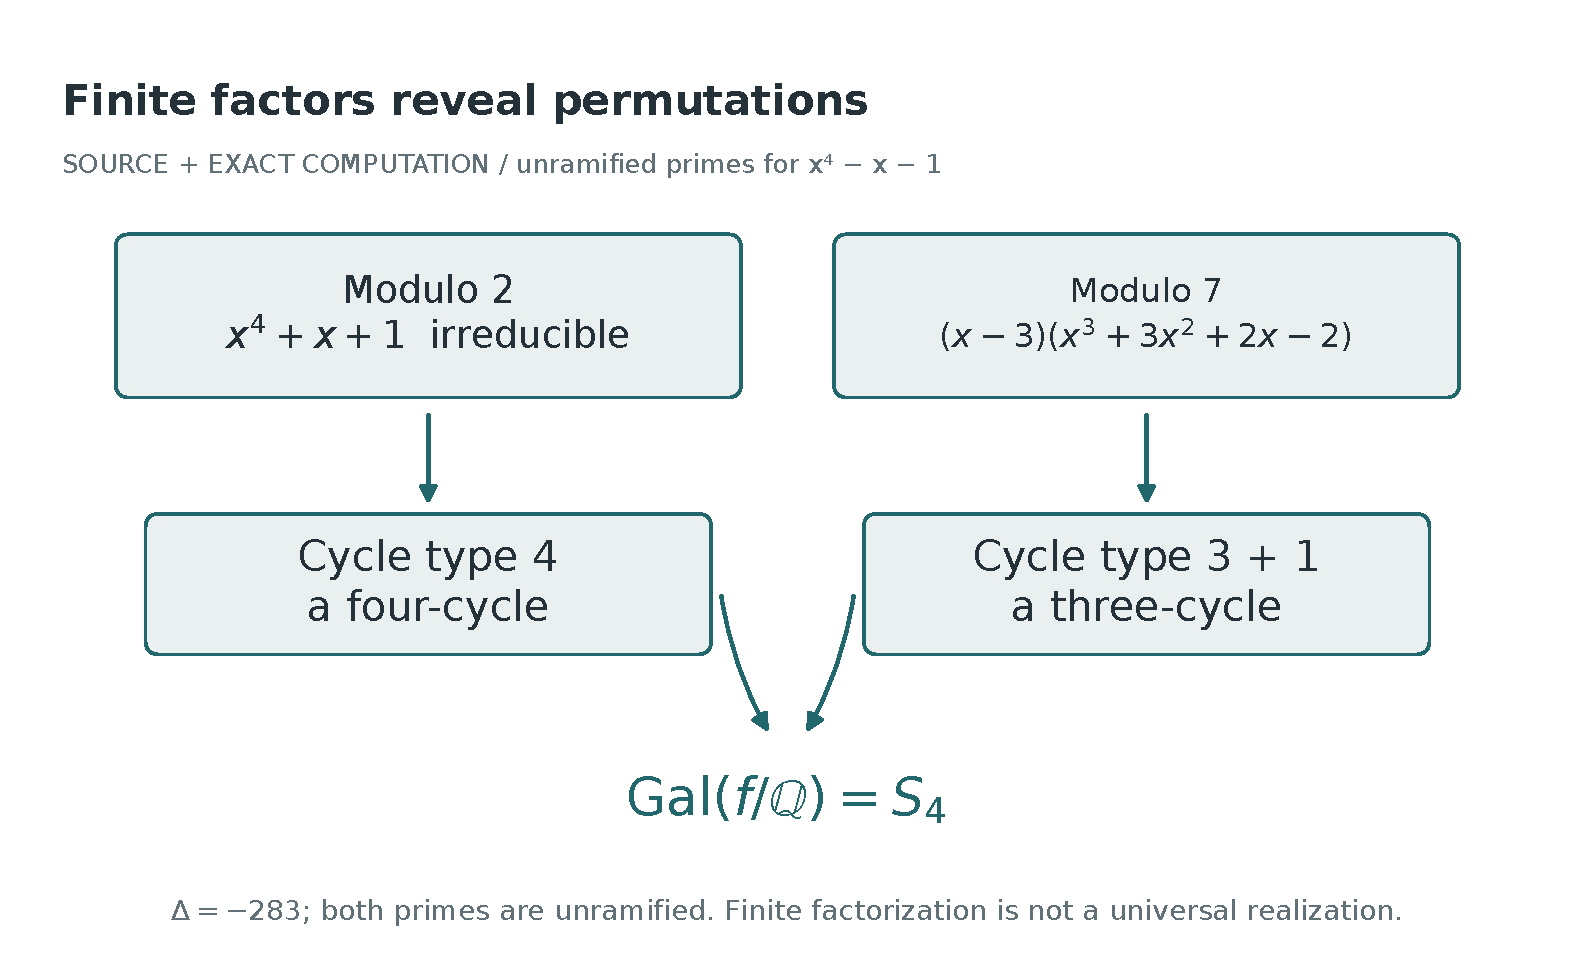
\includegraphics[width=0.96\linewidth]{../visual/figures/07_factor_cycle.pdf}
\caption{The modular certificates for $X^4-X-1$ produce a four cycle at two and a three cycle at seven. Squarefreeness is checked at both primes. A short subgroup argument then identifies the characteristic zero group as $S_4$. These two exact prime calculations certify this polynomial, not a family of arbitrary groups.}
\label{fig:g02-factor-cycle}
\end{figure}

Let $H$ be the Galois group in its faithful action on four roots. Its order is divisible by four and three, so it is divisible by twelve. Since $H\le S_4$, its order is twelve or twenty four. A subgroup of order twelve would have index two and would be normal. The quotient map $S_4\to C_2$ would send all transpositions to the same element because they are conjugate. They generate $S_4$, so this element must be nontrivial. Its kernel is therefore exactly $A_4$, the permutations expressible as a product of an even number of transpositions. But a four cycle is odd. Since $H$ contains one, $H$ cannot be $A_4$. It follows that $H=S_4$.

\begin{resultbox}
The fields above realize $C_2$, $V_4$, $C_3$, $S_3$ and $S_4$ over $\Q$. Each conclusion has a finite, complete proof. The quartic proof imports the good prime cycle theorem and combines it with explicit factorization checks and a proved subgroup argument.
\end{resultbox}

These examples answer five individual existence questions. Their value is not a numerical extrapolation to all finite groups. They make the required ingredients visible: an actual field, controlled degree, full root closure and enough information to identify the entire group. A general construction has to furnish counterparts of those ingredients for an arbitrary prescribed $G$.

\chapter{Every group acts on a field, but the base changes}
\label{chap:g03-generic}

\section{Independent variables keep the action faithful}

Fix a finite group $G$. For every $g\in G$, introduce an independent variable $x_g$. Let
\[
E=\Q(x_g\mid g\in G)
\]
be the rational function field in these $|G|$ variables. Algebraic independence means that no nonzero polynomial with rational coefficients in the $x_g$ vanishes. In particular distinct variables are distinct elements of $E$.

For $h\in G$, define
\begin{equation}
\label{eq:g03-variable-action}
\sigma_h(x_g)=x_{hg},\qquad\sigma_h(q)=q\quad(q\in\Q).
\end{equation}
A permutation of independent variables extends to an automorphism of the polynomial ring and then of its fraction field. The inverse is $\sigma_{h^{-1}}$. The action satisfies $\sigma_h\sigma_k=\sigma_{hk}$, so it is a group action by genuine field automorphisms. It is faithful because $\sigma_h(x_1)=x_h$ differs from $x_1$ when $h\ne1$.

Let
\[
K=E^G=\{z\in E:\sigma_h(z)=z\text{ for every }h\in G\}.
\]
This is a field containing $\Q$. Unlike the vector space model in Chapter~\ref{chap:g01-question}, we now have field multiplication and a faithful action preserving it. The finite automorphism theorem can therefore be applied with its actual hypotheses satisfied.

\begin{figure}[tbp]
\centering
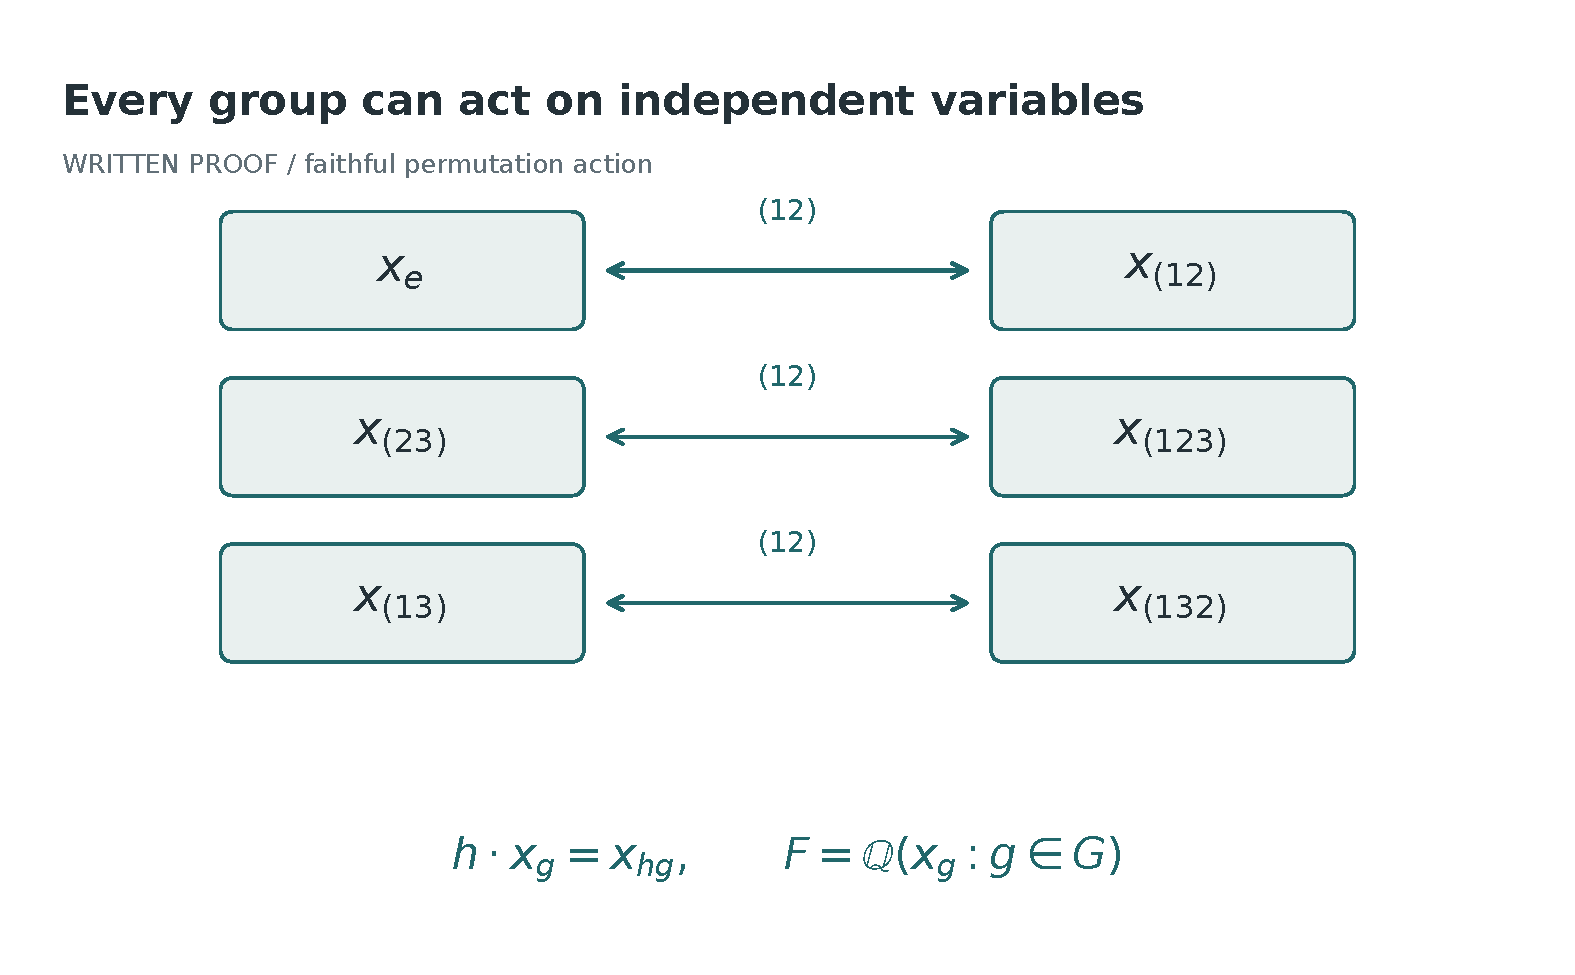
\includegraphics[width=0.96\linewidth]{../visual/figures/08_generic_variables.pdf}
\caption{Independent variables turn the left regular permutation action into an action by field automorphisms. The diagram illustrates multiplication by $(12)$ in $S_3$ and writes $F$ for the field called $E$ in the text, with $e=1$ for the group identity. Artin's theorem realizes the group over its fixed field $K$, while the required arithmetic base remains $\Q$.}
\label{fig:g03-variables}
\end{figure}

\section{The fixed field theorem and its exact conclusion}

\begin{theorem}[Artin's finite automorphism theorem, external input]
\label{thm:g03-artin}
Let $E$ be a field and $A$ a finite subgroup of $\Aut(E)$. If $K=E^A$, then $E/K$ is a finite Galois extension,
\[
[E:K]=|A|,
\qquad
\Gal(E/K)=A.
\]
\end{theorem}

The theorem, with no finiteness assumption on $E$ over some preassigned smaller field, is the classical finite automorphism theorem \cite[Corollary 3.11]{Milne2022}. Its important finiteness condition is on the acting subgroup $A$. It is not a theorem about an arbitrary infinite group of automorphisms.

Applied to~\eqref{eq:g03-variable-action}, it gives
\begin{equation}
\label{eq:g03-generic-extension}
\Gal(E/K)\simeq G,
\qquad
[E:K]=|G|.
\end{equation}
This is a universal realization over a group dependent field $K$. It proves that no finite abstract group is incompatible with field automorphism structure. It leaves the chosen arithmetic base untouched.

An orbit polynomial gives a useful piece of the theorem's mechanism. For any $a\in E$,
\[
P_a(T)=\prod_{h\in G}(T-\sigma_h(a))
\]
has coefficients in $K$, since the action permutes its factors. Thus every element of $E$ is algebraic over $K$. Orbit repetitions are allowed, so this polynomial need not be the minimal polynomial and can have repeated factors. The fact that all such elements together generate a finite extension of degree exactly $|G|$ is the content of Artin's theorem. Bounded degrees for individual elements should not be substituted for that theorem without a further argument.

In our particular construction, $a=x_1$ has $|G|$ distinct images. The polynomial
\begin{equation}
\label{eq:g03-orbit-polynomial}
P(T)=\prod_{g\in G}(T-x_g)
\end{equation}
has degree $|G|$ and coefficients in $K$. Any polynomial over $K$ vanishing at $x_1$ vanishes at every $x_g$ after applying the automorphisms. It therefore has at least $|G|$ distinct roots. The minimal polynomial of $x_1$ has degree $|G|$. In view of~\eqref{eq:g03-generic-extension},
\[
E=K(x_1).
\]
This establishes a primitive element explicitly for the generic extension. The labels on its roots still encode the regular action.

\section{Why the invariant base is not $\Q$}

Already the invariant
\[
s=\sum_{g\in G}x_g
\]
is transcendental over $\Q$. If a nonzero polynomial $F\in\Q[T]$ satisfied $F(s)=0$, then $F(\sum_gx_g)$ would be a zero polynomial in independent variables. Substituting zero for every variable except $x_1$ would give the impossible identity $F(x_1)=0$. Thus $s\in K\setminus\Q$.

More generally, $E/K$ is algebraic, so the two fields have the same transcendence degree over $\Q$:
\begin{equation}
\label{eq:g03-transdegree}
\operatorname{trdeg}_{\Q}K=\operatorname{trdeg}_{\Q}E=|G|.
\end{equation}
The finite degree $[E:K]$ does not make $E$ or $K$ finite over $\Q$. Both retain transcendental parameters. For the trivial group, the construction says only that $E=K=\Q(x_1)$, whereas its arithmetic realization was simply $\Q$. Even this endpoint shows why changing the base cannot be silently ignored.

There is another issue. Knowing the transcendence degree of $K$ does not prove that $K$ is a rational function field. A field of transcendence degree $d$ can be a nontrivial algebraic extension of $\Q(t_1,\ldots,t_d)$. The assertion that a particular invariant field is purely transcendental is a separate rationality problem, commonly called Noether's problem for this action. It must be supplied or proved for the group under consideration. Milne reports Swan's counterexample to universal rationality for the usual permutation action \cite[Aside 5.41]{Milne2022}. We have not independently audited Swan's original counterexample. This is source attributed context and is not a dependency of the conditional realization argument below. Failure of rationality for a group would not rule out a different inverse Galois construction.

\begin{figure}[tbp]
\centering
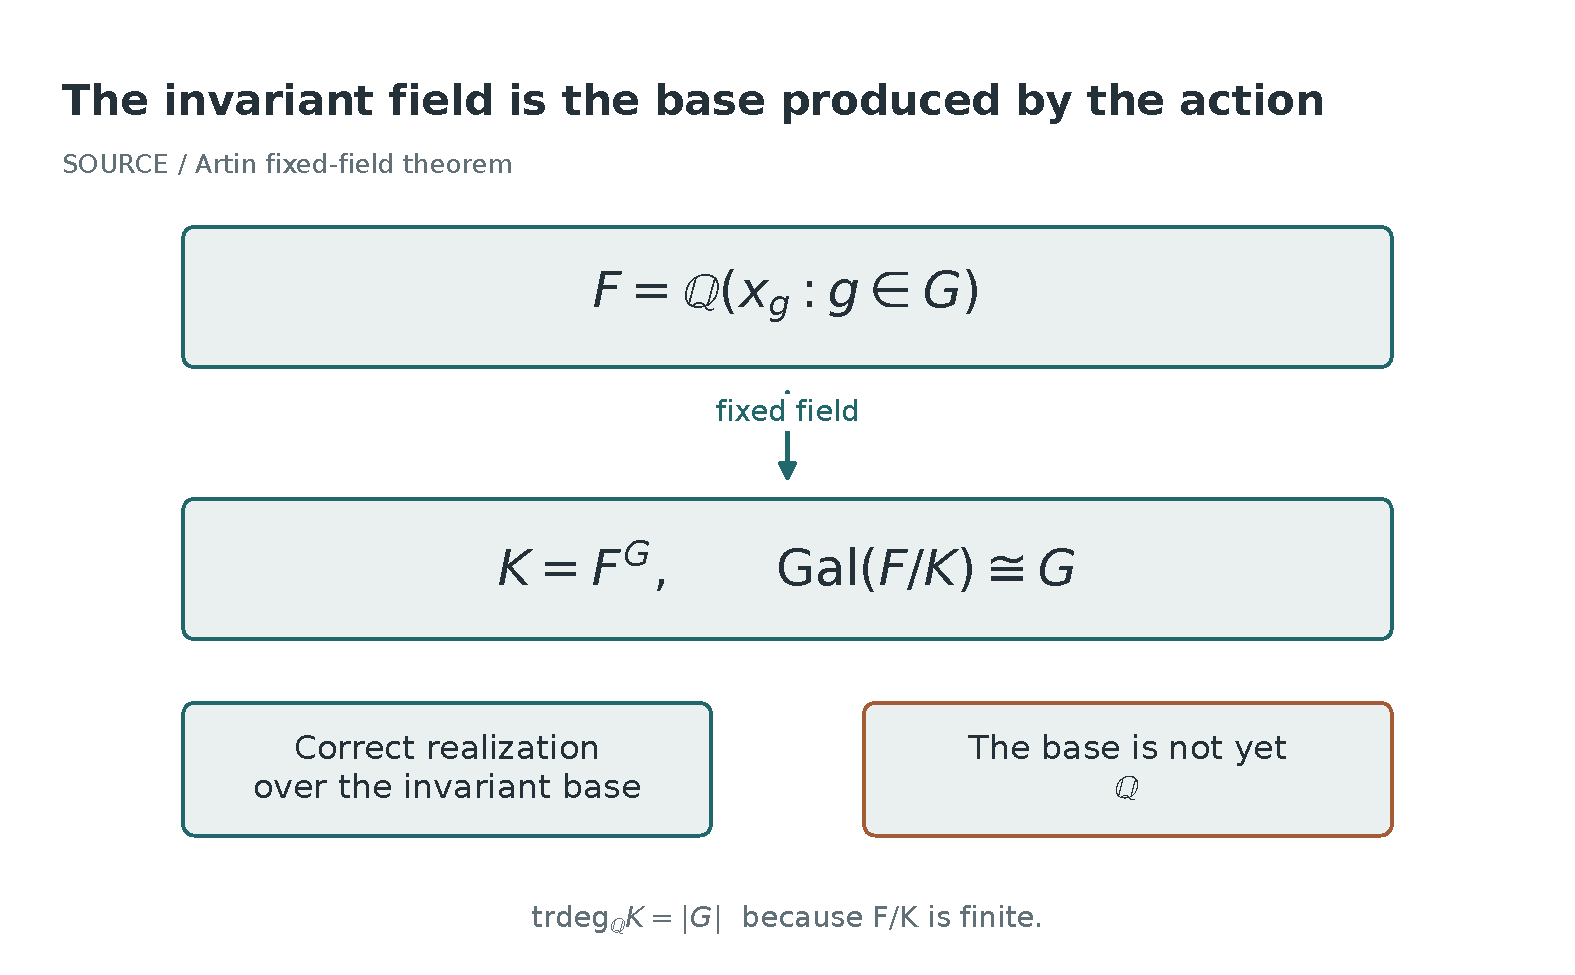
\includegraphics[width=0.96\linewidth]{../visual/figures/09_invariant_base.pdf}
\caption{The invariant field contains rational constants and also transcendental invariants. The diagram writes $F=E$ and $K=F^G$. Its transcendence degree is fixed by the finite extension $E/K$. Pure transcendence requires an additional rationality argument before Hilbert specialization can be applied through a rational parameter presentation.}
\label{fig:g03-invariant-base}
\end{figure}

\section{A sufficient rationality route}

\begin{definition}
An extension $E/\Q(t_1,\ldots,t_d)$ is regular over $\Q$ if every element of $E$ algebraic over $\Q$ belongs to $\Q$. In the characteristic zero setting considered here, this is the constant field condition used for regular finite Galois extensions.
\end{definition}

Our rational function field $E=\Q(x_g)$ has this property. To see the constant field assertion directly, suppose $r\in E$ is algebraic over $\Q$. Write $r=A/B$ for polynomials over $\Q$ with $B\ne0$. There is a rational tuple at which $B$ is nonzero: a nonzero polynomial over the infinite field $\Q$ cannot vanish on every rational tuple, by induction on the number of variables. A monic minimal polynomial $m\in\Q[T]$ satisfies $m(A/B)=0$ identically. Evaluating at that tuple gives a rational root of $m$. Irreducibility forces $m$ to have degree one, so $r\in\Q$.

\begin{theorem}[Hilbert specialization, external input]
\label{thm:g03-hilbert}
Let $d\ge1$ and let $E/\Q(t_1,\ldots,t_d)$ be a finite regular Galois extension with group $G$. There is a Hilbert subset of rational parameter tuples for which specialization is defined and the specialized extension has full Galois group $G$. The tuples may be required to avoid the zero set of any prescribed nonzero polynomial that records finitely many excluded denominators or discriminants.
\end{theorem}

This form combines the specialization theorem with Hilbert irreducibility and its Zariski density statement for rational Hilbert subsets \cite[Theorem 2.6.3, Theorem 5.2.4 and Proposition 5.2.14]{DebesLectureNotes}. It is an imported arithmetic theorem. The phrase ``full group'' is substantive. Outside an exceptional algebraic locus, a specialization can still have a proper subgroup. Hilbert irreducibility provides parameters retaining the needed irreducibility and hence the full degree, not merely parameters at which a polynomial remains defined.

\begin{proposition}[Rational invariant field is sufficient]
\label{prop:g03-noether-route}
For the regular variable action above, suppose the invariant field has a rational presentation
\[
K=\Q(t_1,\ldots,t_d)
\]
with algebraically independent $t_1,\ldots,t_d$. Then $G$ occurs as a Galois group over $\Q$.
\end{proposition}

\begin{proof}
By~\eqref{eq:g03-transdegree}, $d=|G|$, so $d\ge1$. Artin's theorem gives a finite Galois extension $E/K$ with group $G$. The preceding constant field argument proves that $E$ is regular over $\Q$. With the assumed presentation of $K$, all hypotheses of Theorem~\ref{thm:g03-hilbert} hold. A full group specialization gives a finite Galois extension of $\Q$ with group $G$.
\end{proof}

The proposition is a sufficient implication. It does not say that every realization over $\Q$ must come from this particular invariant field or that inverse Galois and Noether rationality are equivalent. A different regular construction, or a direct number field construction, may realize a group without resolving this invariant field's rationality. The proof also does not specify effective parameter sizes. An existence theorem for a Hilbert subset is different from a complete practical search algorithm with a prescribed stopping bound.

\section{Specialization can lose symmetry}

The smallest example makes the warning exact. Let $G=C_2$ exchange two variables $x,y$. Define
\[
s=x+y,\qquad p=xy.
\]
The variables $x,y$ are the roots of $T^2-sT+p$. Since $y=s-x$, the field $\Q(x,y)$ has degree at most two over $\Q(s,p)$. The nontrivial exchange fixes $s,p$, and $x\notin\Q(s,p)$ because an element in that field would be fixed. Hence the degree is exactly two. Artin's theorem then shows
\[
\Q(x,y)^{C_2}=\Q(s,p).
\]
The parameters $s,p$ are algebraically independent: the algebraic extension to $\Q(x,y)$ preserves transcendence degree two.

At $(s,p)=(0,-2)$ the polynomial becomes $T^2-2$, giving the quadratic realization already proved. At $(s,p)=(0,-1)$ it becomes $T^2-1$ and splits over $\Q$, so its splitting field has trivial group. Both discriminants are nonzero, respectively eight and four. Avoiding collisions alone therefore does not preserve the group. At $(s,p)=(2,1)$ the polynomial is $(T-1)^2$, which also fails separability. This is why a full group Hilbert specialization requires more than a nonzero discriminant.

\begin{openproblem}
For an arbitrary finite group, the variable action constructs a Galois extension over its invariant field. To turn this route into a realization over $\Q$, one must provide a suitable rational base presentation or another arithmetic construction. No claim that all invariant fields are rational is made here.
\end{openproblem}

The construction has isolated a genuine obligation. Symmetry is exact, the field is genuine, and the extension degree over the invariant base is known. What remains in this route is the passage to a suitable arithmetic base. The later chapters place that obligation beside the projector and packet language recovered from Operation Komorebi's earlier work.
